\documentclass[../main.tex]{subfiles}
\graphicspath{{\subfix{../images/}}}
\begin{document}
\section*{Term 1 Week 4}
\begin{enumerate}
    \item 
    The answer is not 3. It is 4, although that does depend on how you define \textit{revolution}.\\

    Link here:\\
    \href{https://www.youtube.com/watch?v=FUHkTs-Ipfg&ab_channel=Veritasium}{The SAT question that everybody got wrong}

    \item 
    Find the area of the red square.\\
    \begin{figure}[H]
        \centering
        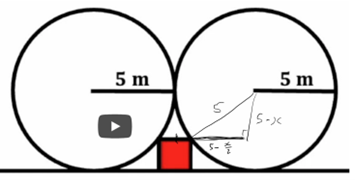
\includegraphics{images/t1w4q2_a.png}
    \end{figure}

    \((5-\frac{x}{2})^2+(5-x)^2=25\)\\

    \(25-5x+\frac{x^2}{4}+25-10x+x^2=25\)\\

    \(\frac{5x^2}{4}-15x+25=0\)\\

    \(5x^2-60x+100=0\)\\

    \(x^2-12x+20=0\)\\

    \(x=2,10\)\\

    Since x must be less than 5m, it cannot equal 10. Therefore, x=2 and the area of the square is 4m\(^2\).\\
    
    \item 
    Take log base 3 of both sides:\\
    \(\log_3 2^x=\log_5 2\)\\

    \(x \log_3 2=\log_5 2\)\\

    \(x=\frac{\log_5 2}{\log_3 2}\)\\

    Using the change of base formula, we know that \(\log_3 2=\frac{\log_5 2}{\log_5 3}\)\\

    \(x=\frac{\log_5 2}{\frac{\log_5 2}{\log_5 3}}=\log_5 2 \times \frac{\log_5 3}{\log_5 2}=\log_5 3\)
\end{enumerate}

\end{document}



